\documentclass[UTF8]{article}

%--
\usepackage{ctex}
\usepackage[margin=1in]{geometry}
\usepackage{graphicx}
\usepackage{subfigure}

%--
\begin{document}
    
%--
{\flushleft \bf \Large 主题:} 形式化语言与自动机大作业-图灵机实验报告

{\flushleft \bf \Large 姓名:} 黄彬寓

{\flushleft \bf \Large 学号:} MF20330030

{\flushleft \bf \Large 日期:} 2020.12.18



\section{设计思路}
\subsection{step1.命令行预处理}
根据main的参数argc、argv对命令行做预处理,使得命令行完全匹配./turing [-v|--verbose] [-h|--help] <tm> <input>格式,检查命令行是否合法、文件名是否存在、是否需要输出usage、是否需要进入verbose模式等。这里涉及两个全局变量HELP\_STATE和DEBUG\_STATE,即方便判断输出什么内容。

\subsection{step2.解析器}
在这里,我们读取.tm文件内容,对文件内容进行剖析,必要时返回syntax error的错误信息。

首先读取方式是用getline每次读取一整行,这样不仅可以读取带空格的一整行,且在循环体内每次对line加一可以计算行号,于是方便在verbose中语法错误时指出具体行号。根据分出的行,我们把其分为三类:1.无用行,为长度<2或以``\verb|;|''开头的行,即(temp.length() < 2 || temp[0] == ';');2.除转移函数外的图灵机参数行,即(temp[0] == '\#');3.转移函数行。第一类行直接丢弃,第二类行在第一次文件按行遍历中处理,第三类行在第二次文件按行遍历中处理。分两次读取文件原因是这样的,为了使得在处理转移函数时能够根据图灵机的其他参数如Q、G等直接判断该转移函数是否合法、是否出现了未定义的状态、符号等,进行更好的处理,因为有些.tm文件可能会把转移函数写在其他参数之前,这样的话先读取到转移函数就无法直接对转移函数中的各个状态符号进行判定。

第一次读取文件时处理除转移函数外的其他图灵机参数,即Q、S、G、q0、B、F、N。这里我封装了三个函数,storeStates2QF用于处理Q、F,storeChar2SG用于处理S、G,storeNum2q0BN用于处理q0、B、N,原因是Q、F均为状态集,S、G均为符号集,q0、B、N是三个单变量可相似处理。这三个函数的参数为(int line, string str,string type),line为所在行号,用于verbose模式下遇到语法错误时指定位置,str为改行字符串,type为处理对象,如处理q0时type为"q0"。函数内部即为对整行进行遍历,实现细节各异,但首先需要遍历一遍,若遇到``\verb|;|''则只取该位置之前的字符串。接着就是对各个字符串进行详细处理,并存入图1这样的数据结构中,这里过于冗杂不做说明,大部分的syntax error均在这三个函数内做输出。剩下一些syntax error需要等这些参数全部设置完后才能进行判断,如S是否尚未被定义、S是否被重定义、B是否在G中、S中的每个元素是否都在G中等。
\begin{figure}[h]
  \centering
  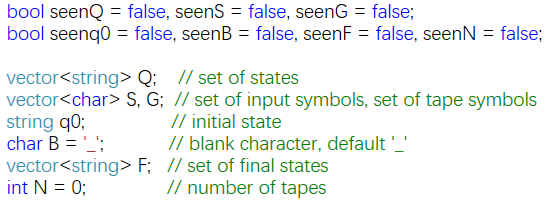
\includegraphics[scale=0.6]{pic1.png}
  \caption{图灵机中除转移函数外参数的定义}
 %% \Description{This is an example of list in distributed systems.}
\end{figure}

第二次读取文件时处理转移函数,因为此时其他参数均以设置好,所以剩下的syntax error可以在处理转移函数时全部完成判断,如每个符号是否在G中存在,某个状态是否在Q中被定义等。这里我封装了一个函数storeItem2delta,参数为(int line, string str),line同样用于出错时打印行号。这里我设置一个五元组string ele[5],依次将旧状态、旧符号集、新符号集、方向组、新状态存入,若不满5个或超过5个均为语法错误。
\begin{figure}[h]
  \centering
  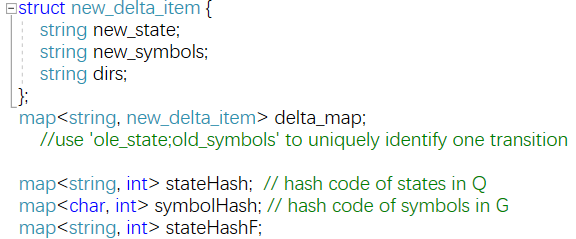
\includegraphics[scale=0.6]{pic2.png}
  \caption{图灵机中转移函数定义及其他加快计算的哈希表}
 %% \Description{This is an example of list in distributed systems.}
\end{figure}
这里我的数据结构如图2所示,使用哈希表是为了加快计算,思想是这样的,string型的id为``\verb|<old_state>;<old_symbols>|'',因为";"是一个不会出现在状态和磁带符号中的一个字符,用它来做状态和符号的分隔符较为稳妥,且这样一定能够唯一标识某一个转移函数,若找不到则说明在该处停机,若找到则根据表内对应项的新符号、方向组、新状态进行转移即可。

随后解析器部分就基本完成了,最后若DEBUG\_STATE为1代表在verbose模式下,则所有syntax error都在处理过程中输出了,否则不在verbose下在最后输出"syntax error"。这样找到语法错误不急着输出并返回,而在最后才进行判定是因为:一个文件内可能有多处语法错误,如果找到一处错误则输出返回,那么我们可能会丢失很多其他错误的反馈,对debug不利,于是统计所有语法错误,找到一处输出一处其行号和错误信息,最后我们能够在verbose模式下所有存在的语法错误,便于debug。

\subsection{step2.模拟器}
在这部分,首先需要判断输入串的合法性 ,也即判断所有字符是否均属于输入符号集,于是专门用一个judgeInput函数来进行处理,若在verbose模式下则额外输出出错的那些符号及相应下标位置。

随后在模拟器模块,首先我们定义磁带、每条磁带的指针下标、当前状态等一系列数据,随后进入主循环体,每一次循环内都是由上一个状态到下一个状态的一次转移。首先判断在图2中的stateHashF中是否存在当前状态,若存在则说明这是终止状态,跳出循环并输出程序以接受方式结束,判断条件即if (stateHashF.count(cur\_state) \&\& stateHashF[cur\_state] > 0);否则,获取当前状态及每条磁带指针所指向的符号,构成图2中的delta\_map的索引,id为``\verb|<old_state>;<old_symbols>|'',判断条件即(delta\_map.count(id)),若找不到则说明在该状态和符号组下没有相应的转移函数,跳出循环并输出程序以停机方式结束;否则说明找到了相应的转移函数,则根据delta\_map[id]结构体内的新符号组、方向组和新状态对当前状态、磁带指针指向符号、指针位置进行修改,进行下一轮循环。

在这里,若是verbose模式下,需要打印出每个step的具体细节,我们额外定义一个数据结构用于找到每条磁带当前有效区间的两端下标,来辅助输出信息,这里按部就班编写就可以,唯一需要注意的是head打印位置,这里我为了方便打印head位置,将原本的一边遍历一边打印换成了先预先存在字符串中最后一起打印,然后当遍历到当前磁带的指针下标时,用一个tag记录当前index那条字符串的长度,这样打印head位置的时候只需要在tag标识的位置打印即可。

\subsection{多带图灵机程序}
程序一:(多种转向false的情况过于冗杂不详述,可直接看原码)

1.使用两条磁带,两个指针分别右移,将第一条磁带的前半部分a+b+串存入第二条磁带,并在第一条磁带上删除。

2.此时两指针均在各自ab串的头部,于是指针分别后移并判断每一位是否相等。

3.此时若成功,则第一条磁带内容为空,写入true即可;若失败,则首先将第一条磁带指针不断右移置为空,然后写入false即可。

程序二:(多种转向false的情况过于冗杂不详述,可直接看原码)

1.使用三条磁带,将第一条磁带中的第一部分的1串写入第二条磁带,并在第一条磁带中删除。

2.将第一条磁带中的第二部分的1串写入第三条磁带,并在第一条磁带中删除。

3.此时第二、第三条磁带的指针位于串的尾部,将它们的指针左移指向1串的头部。

4.重复一个过程:若第二条磁带指针指向1,将第二条磁带右移一位,第一条磁带和第三条磁带的指针同步右移,当第三条磁带指针指向空,将其左移到初始头部,然后进入下一次循环过程。过程中当三个指针均第一次同时指向空时成功,失败情况过多可直接看原码。

5.成功时,第一条磁带内容必为空,直接写入true即可;失败时,则首先将第一条磁带指针不断右移置为空,然后写入false即可。


\section{实验完成度}   
解析器模块错误处理和选作部分、模拟器模块、多带图灵机程序全部完成。

\subsection{预处理部分}
\begin{figure}[h]
  \centering
  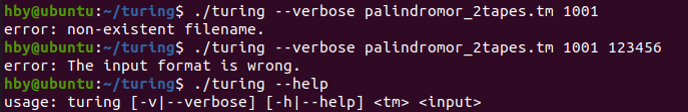
\includegraphics[scale=0.8]{pic4.png}
  \caption{预处理部分结果显示}
 %% \Description{This is an example of list in distributed systems.}
\end{figure}

\subsection{解析器部分:参数Q、F可检测的syntax error}

\begin{itemize}
    \item 缺失'=',syntax error: Line <line>, miss character '=' before '\{'.  
    \item 缺失'\{',syntax error: Line <line>, miss character '\{'.  
    \item 两个逗号或逗号与括号间无符号或仅含空格时,syntax error: Line <line>, there exists a state whose identifier is blank in <Q/F>.
	\item 状态中含有除规定外的其他字符,syntax error: Line <line>, unrecognized character in identifier of state in <Q/F>. 
    \item 缺失'\}',syntax error: Line <line>, miss character '\}'.
    \item 在'\}'后还有除注释外的其他内容,syntax error: Line <line>, there exists something else after the character '\}'.
	\item 重定义,syntax error: Line <line>, <Q/F>  is re-defined.
    \item 尚未定义,此时因为没有定义所以也没有行号提示,syntax error: <Q/F> is not defined.
\end{itemize}

\subsection{解析器部分:参数S、G可检测的syntax error}
\begin{itemize}
    \item 缺失'=',syntax error: Line <line>, miss character '=' before '\{'.  
    \item 缺失'\{',syntax error: Line <line>, miss character '\{'.  
    \item 两个逗号或逗号与括号间无符号或仅含空格时,syntax error: Line <line>, there exists a symbol whose identifier is blank in <S/G>.
	\item 符号长度超过1时,syntax error: Line <line>, there exists a symbol whose length not equal 1 in <S/G>.
	\item 符号为规定外的符号如';'等,syntax error: Line <line>, disallowed expression of the symbol in <S/G>.
    \item 缺失'\}',syntax error: Line <line>, miss character '\}'.
    \item 在'\}'后还有除注释外的其他内容,syntax error: Line <line>, there exists something else after the character '\}'.
	\item 重定义,syntax error: Line <line>, <S/G>  is re-defined.
    \item 尚未定义,此时因为没有定义所以也没有行号提示,syntax error: <S/G> is not defined.
	\item S中存在未在G中定义的符号,syntax error: Some symbol <symbol> in S is not in G.
\end{itemize}

\subsection{解析器部分:参数q0、B、N可检测的syntax error}
\begin{itemize}
    \item 缺失'=',syntax error: Line <line>, miss character '='.  
    \item 定义后还有除注释外的其他内容,syntax error: Line <line>, there exists something else after the blank symbol B.
    \item 初始状态中含有除规定外的其他字符,syntax error: Line <line>, unrecognized character <character> in identifier of initial state q0.
	\item N不是一个数字,syntax error: Line <line>, <num> is not a digit in tape number N.
	\item N不是一个正自然数,syntax error: Line <line>, tape number N is less than 1 which should not happen.
    \item B不在G中,syntax error: B is not in G.
    \item q0不在Q中,syntax error: q0 is not in Q.
	\item 重定义,syntax error: Line <line>, <q0/B/N>  is re-defined.
    \item 尚未定义,此时因为没有定义所以也没有行号提示,syntax error: <q0/B/N> is not defined.
\end{itemize}

\subsection{解析器部分:参数delta可检测的syntax error}

 \begin{itemize}
    \item 一行中不足5个参数,syntax error: Line <line>, delta has less than 5 arguments which can not construct a delta item.
    \item 一行中超过5个参数,syntax error: Line <line>, delta has more than 5 arguments which exceeds the requirement.
    \item 转移函数中的旧状态不在Q中,syntax error: Line <line>, the old state in delta is not defined in Q.
	\item 转移函数中的新状态不在Q中,syntax error: Line <line>, the new state in delta is not defined in Q.
	\item 旧符号组的长度不为N,syntax error: Line <line>, the length of group of old symbols is not N.
	\item 旧符号组中有某个符号不在G中,syntax error: Line <line>, there exists some symbol not defined in G in group of old symbols.
	\item 新符号组的长度不为N,syntax error: Line <line>, the length of group of new symbols is not N.
	\item 新符号组中有某个符号不在G中,syntax error: Line <line>, there exists some symbol not defined in G in group of new symbols.
	\item 方向组的长度不为N,syntax error: Line <line>, the length of group of directions is not N.
    \item 方向组中有不符合规定的符号,syntax error: Line <line>, there exists some symbol can not be recognized by directions.
\end{itemize}

简单示例:
\begin{figure}[h]
  \centering
  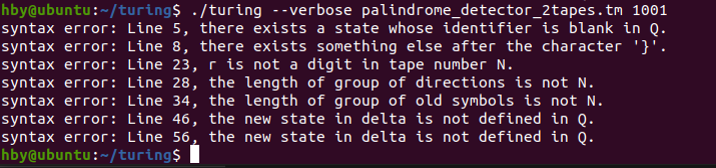
\includegraphics[scale=0.8]{pic5.png}
  \caption{解析器部分结果显示}
 %% \Description{This is an example of list in distributed systems.}
\end{figure}

\subsection{模拟器部分:判断输入串的合法性}
\begin{figure}[h]
  \centering
  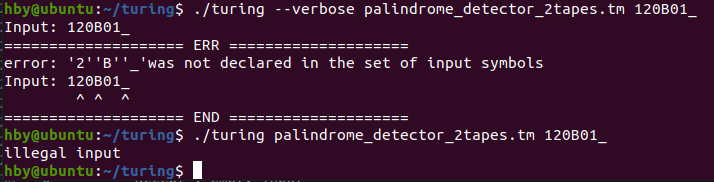
\includegraphics[scale=0.8]{pic6.png}
  \caption{不合法输入串结果显示}
 %% \Description{This is an example of list in distributed systems.}
\end{figure}

\subsection{模拟器部分}
对于输入串进行图灵机模拟,返回结果,并说明是在accept还是halt下结束的,见图6图7。

\begin{figure}[h]
  \centering
  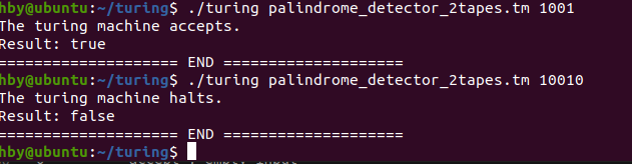
\includegraphics[scale=0.8]{pic7.png}
  \caption{模拟器普通模式显示}
 %% \Description{This is an example of list in distributed systems.}
\end{figure}

\begin{figure}[h]
  \centering
  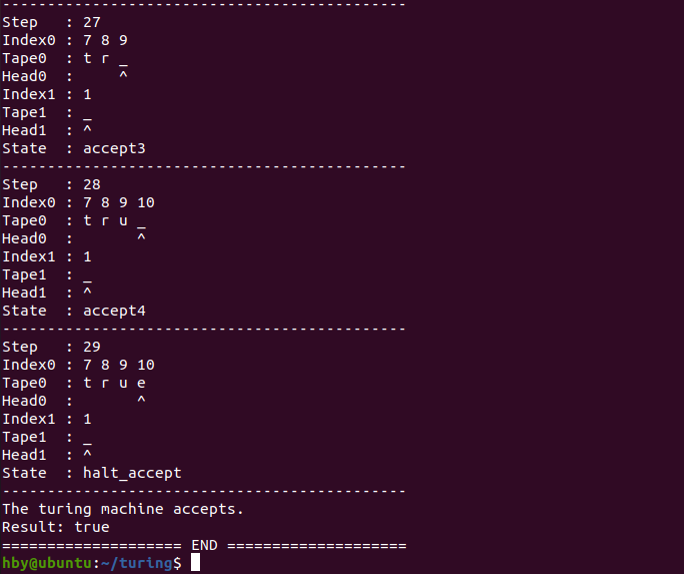
\includegraphics[scale=0.6]{pic8.png}
  \caption{模拟器verbose模式显示}
 %% \Description{This is an example of list in distributed systems.}
\end{figure}

\subsection{用自己的解析模拟器运行case1}
见图8图9。
\begin{figure}[h]
  \centering
  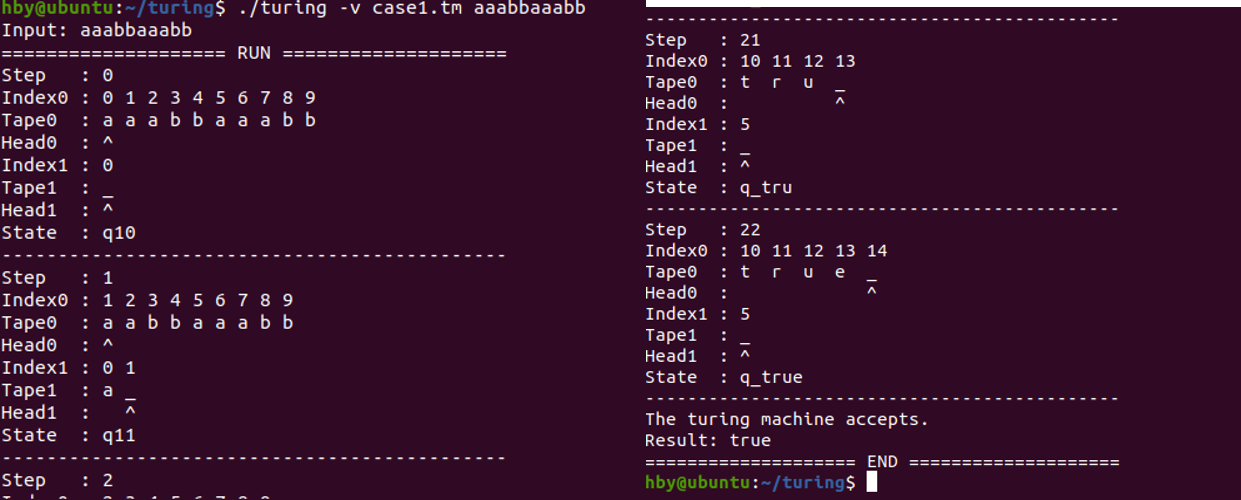
\includegraphics[scale=0.6]{pic9.png}
  \caption{对case1输入为aaabbaaabb下verbose模式输出}
 %% \Description{This is an example of list in distributed systems.}
\end{figure}

\begin{figure}[h]
  \centering
  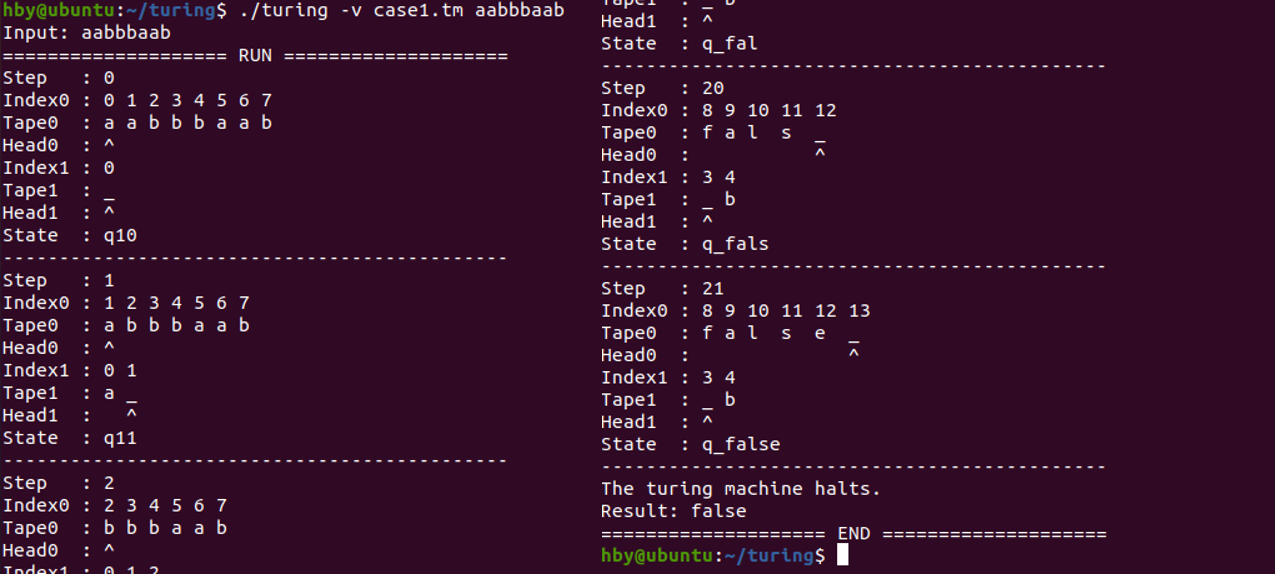
\includegraphics[scale=0.6]{pic10.png}
  \caption{对case1输入为aabbbaab下verbose模式输出}
 %% \Description{This is an example of list in distributed systems.}
\end{figure}

\subsection{用自己的解析模拟器运行case2}
见图10图11。

\begin{figure}[h]
  \centering
  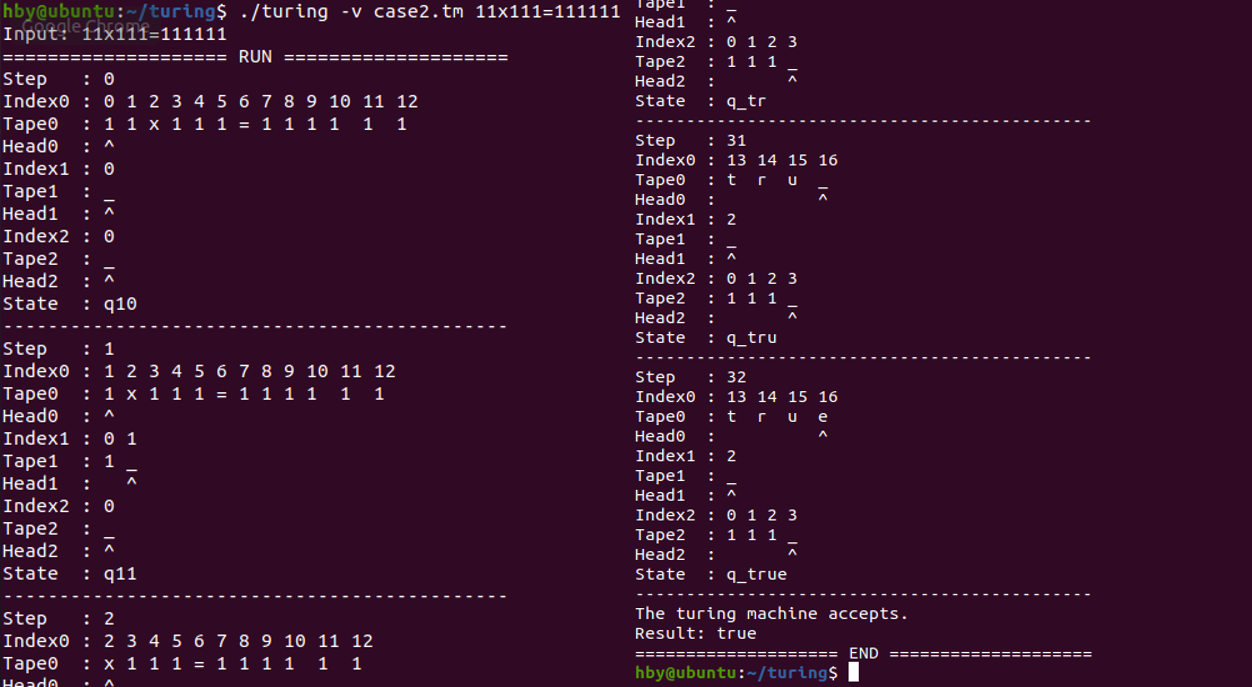
\includegraphics[scale=0.6]{pic11.png}
  \caption{对case2输入为11x111=111111下verbose模式输出}
 %% \Description{This is an example of list in distributed systems.}
\end{figure}

\begin{figure}[h]
  \centering
  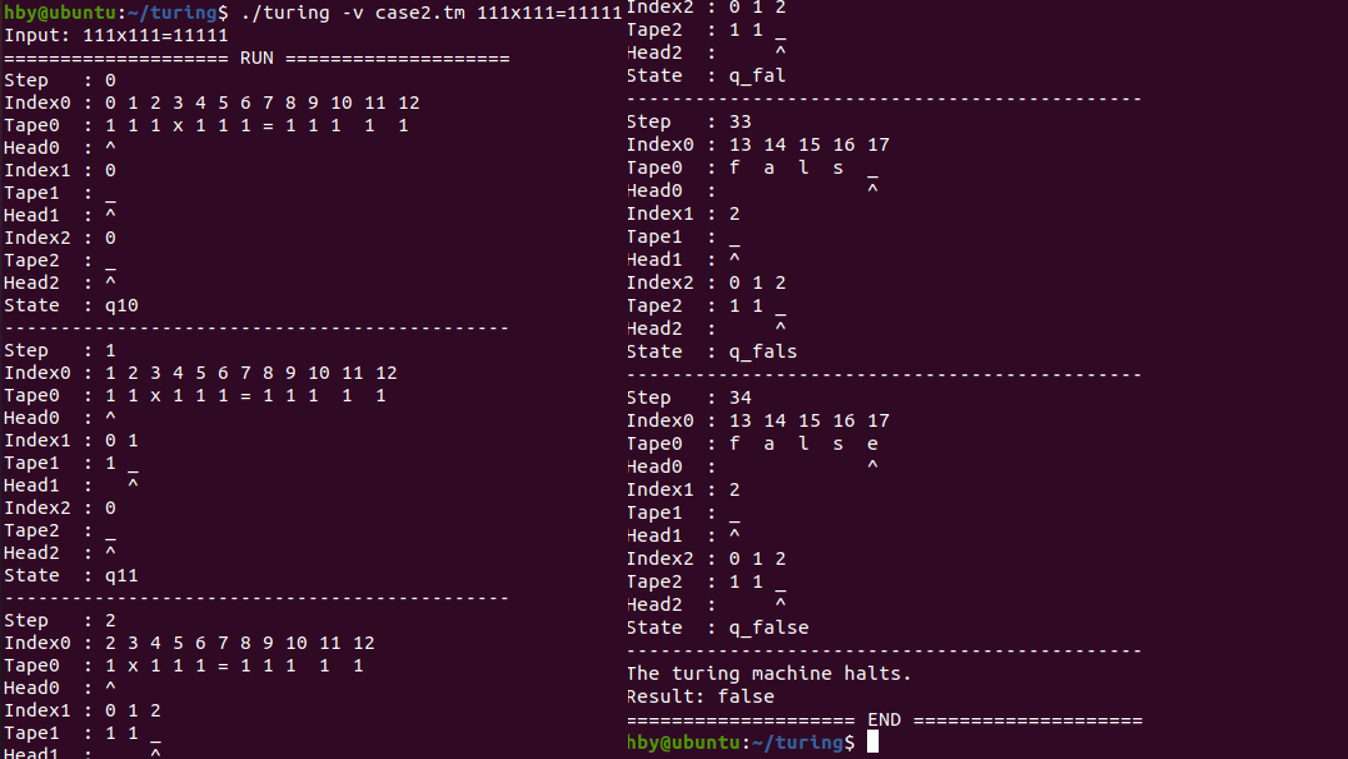
\includegraphics[scale=0.6]{pic12.png}
  \caption{对case2输入为111x111=11111下verbose模式输出}
\end{figure}

\section{遇到的问题及解决方案}
实验过程中主要遇到了两个问题。

第一个问题,在verbose模式下打印内容时,会发现tape输出变为了很多之前打印过的字符串,而并不是我期望磁带上的字符串。经过一段时间的断步调试和在一些关键地方打印数据后,发现了错误在string型变量+char型变量上。我本能的以为string加上某一个char型字符应该与string与string相加同理,但是打印出来发现这个char字符没被加上,而是输出缓冲区中的一部分内容被加了进来导致了输出错误。我把``\verb|output\_tape+=tapes[i][j];|''这条语句修改为``\verb|output_tape.append(1, tapes[i][j]);|''后,bug成功得到修复。

第二个问题,本实验最开始在windows系统下编程和调试完全没问题,后来在Linux中同样的代码,却报出了各种各样的syntax error错误,查看源文件又觉得找不到问题。后来我发现,我是直接把C++文件和.tm文件从windows中拷贝到虚拟机中,于是程序直接对case.tm和case2.tm运行出错,这大概是因为Windows中文件格式和Linux中文件格式转换的问题,Linux中对换行符识别与Windows不一致,于是我在Linux中创建了两个.tm文件,并把内容复制过去再运行新的程序文件,原来的各种syntax error问题就消失了。因此我在programs下放置了case1.tm、case2.tm、case1\_windows.tm、case2\_windows.tm四个文件,前两个是我在Linux下测试过的程序文件,后两个是我在Windows下测试过的程序文件。

\section{总结}
本次实验,任务1由于考虑的各种syntax error情况较多,也带来了一定的编程困难,工作量在500行左右,时间为一天;任务2由于任务1考虑地比较细致,做好了很多准备,编程难度并不高,主要在于向屏幕打印需要花费主要心思,工作量为200行,时间为半天;任务3单纯考虑true的情况逻辑上难度还是比较小的,主要困难在于考虑各种各样的错误情况,并将这些错误情况转移到false状态中,并将第一条磁带清空并打印false是比较麻烦琐碎的,时间为半天。

这次实验让我收获不少,我更加清晰地了解了图灵机的原理以及它的实现流程,并从原来的只了解单带图灵机的视角放宽到了多带图灵机上,让我明白了在一些案例中,使用多带图灵机进行实现会使难度和复杂度降低不少,多带图灵机带来的其余纸袋在存储临时变量或是标记上都有着卓越的优势。

最后很感激这门课的卜磊老师和各位助教,让我更清晰的明白自动机与正则语言、下推自动机与上下文无关语言、图灵机与可判定不可判定问题等,受益良多,而且这些知识对于我的专业课题也有一定的帮助。我的专业中一直用到副本技术,而副本技术内部最常用的就是使用自动机更新内部状态,学习了这门课之后让我对其有了更深的理解。


\end{document}